
\documentclass[tikz,border=7pt]{standalone}
\usepackage[utf8]{inputenc}
\usepackage[T1]{fontenc}
\usepackage{amsmath}
\usepackage{xcolor}
\usetikzlibrary{arrows.meta,calc,angles,quotes,patterns,positioning}
\definecolor{brand}{HTML}{1E3A8A}
\definecolor{brandtwo}{HTML}{2563EB}
\definecolor{accentred}{HTML}{EF4444}
\definecolor{accentgreen}{HTML}{16A34A}
\definecolor{accentorange}{HTML}{F59E0B}
\definecolor{muted}{HTML}{64748B}
\definecolor{lightblue}{HTML}{EEF6FF}
\tikzset{force/.style={-{Latex[length=3mm]}, line width=1.15pt}, axis/.style={-{Latex[length=2mm]}, line width=.8pt, color=muted}, body/.style={draw=brandtwo, fill=lightblue, line width=1pt, rounded corners=2pt}, lab/.style={font=\small, text=brand}, sml/.style={font=\scriptsize, text=muted}}
\begin{document}

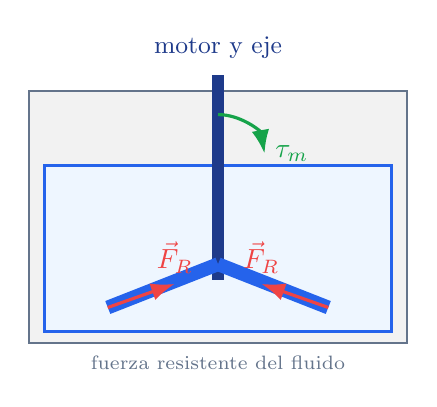
\begin{tikzpicture}[scale=1]
\draw[fill=gray!10, draw=muted, line width=1pt] (-2.4,-.2) rectangle (2.4,3);
\draw[fill=lightblue, draw=brandtwo, line width=1pt] (-2.2,-.05) rectangle (2.2,2.05);
\draw[line width=4pt, color=brand] (0,3.2)--(0,.6);
\draw[line width=5pt, color=brandtwo] (0,.8)--(-1.4,.25); \draw[line width=5pt, color=brandtwo] (0,.8)--(1.4,.25);
\draw[force,color=accentgreen] (0,2.7) arc[start angle=90,end angle=10,radius=.6] node[right] {$\tau_m$};
\draw[force,color=accentred] (1.4,.25)--(.55,.55) node[above] {$\vec F_R$}; \draw[force,color=accentred] (-1.4,.25)--(-.55,.55) node[above] {$\vec F_R$};
\node[lab] at (0,3.55) {motor y eje}; \node[sml] at (0,-.45) {fuerza resistente del fluido};
\end{tikzpicture}

\end{document}